\section{Thématique}\label{sec:objectifs}
\vspace{-2ex}

Au lieu de compléter le cours en complexifiant les circuits logiques réalisés à partir d’un schéma, ce laboratoire tentera plutôt d’aider l’étudiant.e à intégrer des connaissances tout en s’exerçant au raisonnement inductif. Concrètement, l’étudiant.e fera la rétro-ingénierie d’un circuit automatisant la mesure du temps de chute d’une masse avec une emphase sur le conditionnement du signal: cette fonction requiert souvent la conception et fabrication de circuits en recherche expérimentale. On bouclera finalement le cours en revenant à la conversion analogique-numérique avec la conception d’un voltmètre à trois niveaux discrets.

\subsection{Partie 1-Mesure automatisée de l'accélération gravitationnelle}

Cette partie du laboratoire fonctionne un peu en inverse pour développer des aptitudes de rétroingénierie: le montage est déjà fait et vous devez déduire son fonctionnement logique. Chaque équipe disposera d'une vingtaine de minutes avec le montage, veuillez vous adresser à votre équipe d'enseignement pour coordonner l'accès. L'expérience sera consignée dans un seul et même cahier de laboratoire pour toute la classe. Ce cahier pourra alors assumer sa fonction 
tour de rôle partir des notes des précédent


Ce montage sert à mesurer l'accélération gravitationnelle à partir de la chute d'une bille. En fait, il compte le nombre d'oscillations envoyées par un oscillateur entre les événements «de départ» et «d'arrivée», duquel le temps de chute peut être déduit. L'idée générale du montage est illustrée à la figure~\ref{fig:calcul-g}.
\begin{figure}[h]
\centering
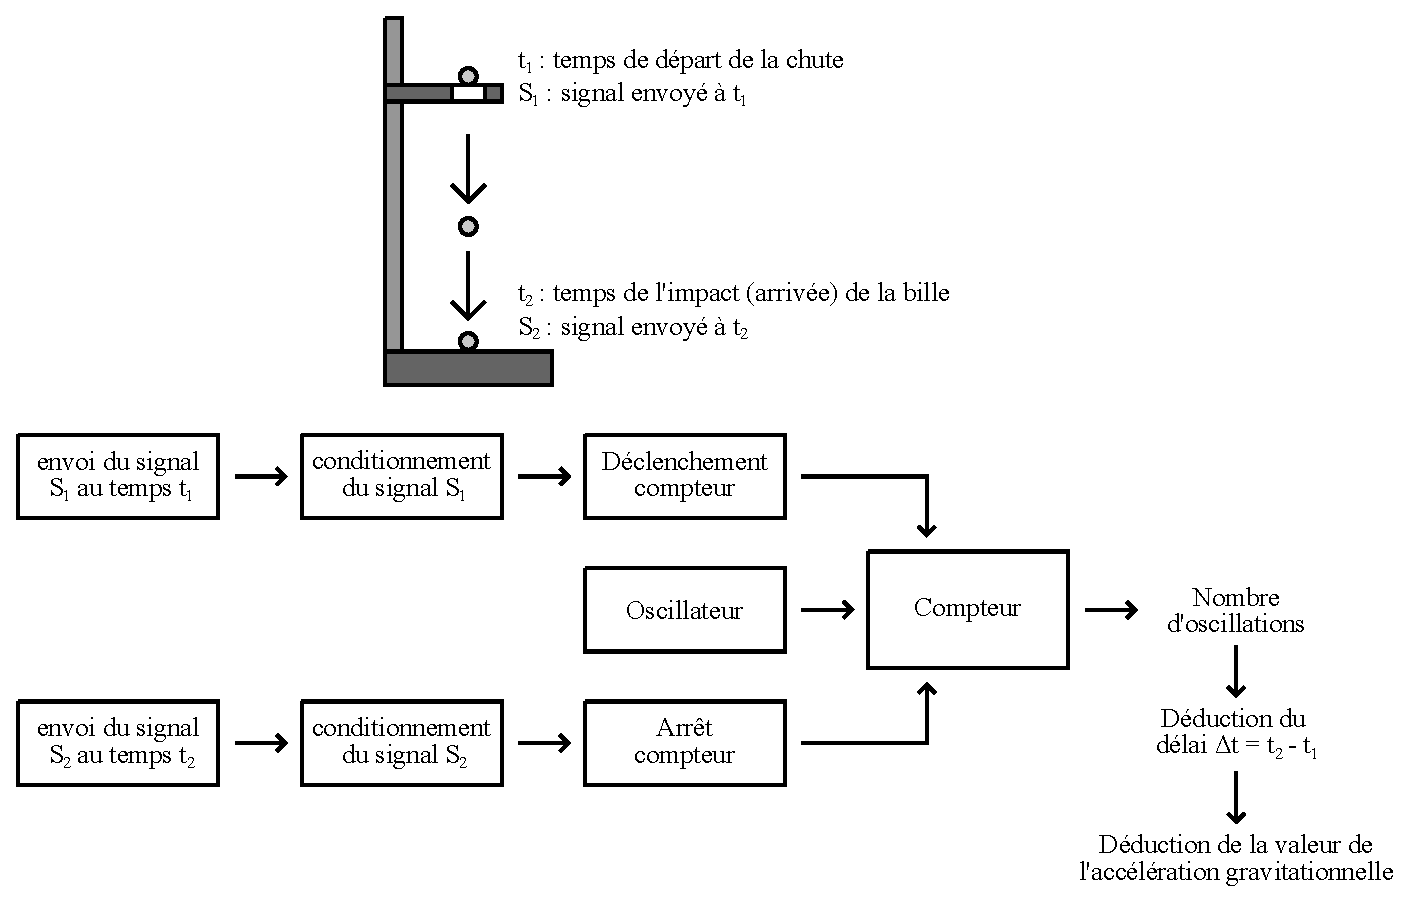
\includegraphics[width=\textwidth]{SchemaFonct-calcul-g}
\caption{\label{fig:calcul-g}Schéma conceptuel illustrant le fonctionnement général du montage servant à déduire l'accélération gravitationnelle.}
\end{figure}

Les manipulations pour cette partie ne sont pas explicitées dans ce protocole. Vous aurez donc à utiliser les fiches techniques des circuits intégrés, un oscilloscope, toute la puissance de votre matière grise, ainsi que l'expérience indéniable que vous avez acquise jusqu'à maintenant, afin de déterminer et de réaliser les manipulations nécessaires. Vos buts sont de comprendre en détail le fonctionnement du circuit et de mesurer l'accélération gravitationnelle en justifiant l'incertitude estimée.

À la fin du deuxième tour, vous devrez expliquer brièvement comment le circuit parvient à effectuer les fonctions suivantes:
\begin{enumerate}
    \item le conditionnement du signal $S_1$ (signal produit par le début de la chute de la bille);
    \item le conditionnement du signal $S_2$ (signal produit par l'impact de la bille);
    \item la génération d'un signal à fréquence fixe;
    \item le déclenchement et l'arrêt du compteur.
\end{enumerate}

Complétez l'expérience en écrivant au tableau votre résultat de mesure d'accélération gravitationnelle pour bâtir une distribution statistique avec vos collègues.